\section{Inserting Vertices}
\label{sect:inserting-vertices}

When a new cluster appears in our underlying data set, we want to add a new vertex to the cluster graph. We distinguish between adding a new vertex on the inside and adding a new vertex on the outside because different rules apply.



\paragraph{Inserting Vertices Inside}

All internal faces of the cluster graph are triangles. If we add a vertex in one of the triangular faces, we must also add edges to the three vertices bounding the face without introducing edge crossings in order to preserve the graph's internal triangulatedness. A valid vertex insertion into an internal face is illustrated in \cref{fig:insert-vertex-inside-example}.

\begin{figure}[H]
	\centering
	\subfigure[]{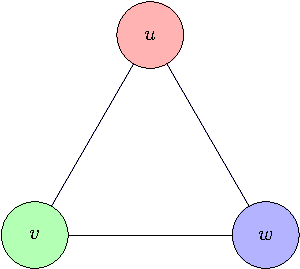
\includegraphics[height=29mm]{Resources/InsertVertexInside-Example-1.pdf}}
	\quad
	\subfigure[]{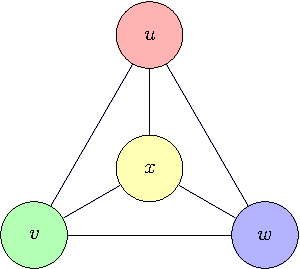
\includegraphics[height=29mm]{Resources/InsertVertexInside-Example-2.pdf}}
	\qquad
	\subfigure[]{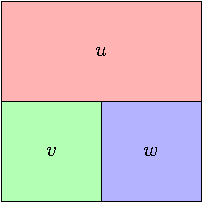
\includegraphics[height=29mm]{Resources/InsertVertexInside-Example-3.pdf}}
	\quad
	\subfigure[]{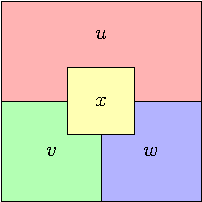
\includegraphics[height=29mm]{Resources/InsertVertexInside-Example-4.pdf}}
	\caption{A cluster graph and a polygonal dual thereof, before (a, c) and after (b, d) inserting the vertex $x$ in the triangular face $uvw$.}
	\label{fig:insert-vertex-inside-example}
\end{figure}

Let $u$, $v$, and $w$ be the vertices bounding an internal face of the cluster graph in counterclockwise order and $x$ the new vertex we want to add inside said face. We compute the paths that form the $u$-$v$-, $v$-$w$-, and $w$-$u$-boundaries in the polygonal dual. Let $p_{uvw}$ denote the vertex where the three faces corresponding to $u$, $v$, and $w$ meet. Let $p_{uv}$, $p_{vw}$, and $p_{wu}$ denote the first subdivision vertex on the boundary between faces $u$ and $v$, $v$ and $w$, and $w$ and $u$, respectively, starting from $p_{uwv}$. If one of the boundaries consist of only one edge, we place a subdivision vertex at its midpoint first. \Cref{subfig:insert-vertex-inside-illustration-1} shows how these vertices might look for the example from above.

\begin{figure}[H]
	\centering
	\subfigure[]{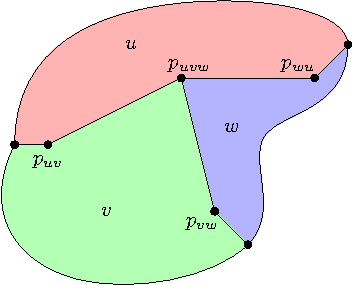
\includegraphics[width=45mm]{Resources/InsertVertexInside-Illustration-1.pdf}\label{subfig:insert-vertex-inside-illustration-1}}
	\quad
	\subfigure[]{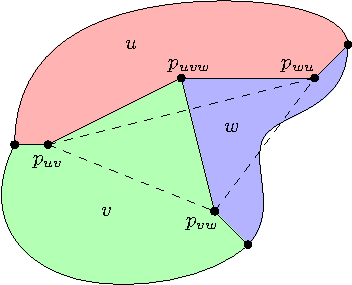
\includegraphics[width=45mm]{Resources/InsertVertexInside-Illustration-2.pdf}\label{subfig:insert-vertex-inside-illustration-2}}
	\quad
	\subfigure[]{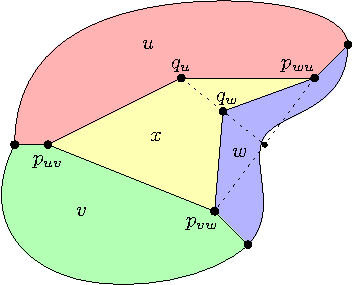
\includegraphics[width=45mm]{Resources/InsertVertexInside-Illustration-3.pdf}\label{subfig:insert-vertex-inside-illustration-3}}
	\caption{Inserting an internal face $x$ at the point where three faces $u,v,w$ meet.}
	\label{fig:insert-vertex-inside-illustration}
\end{figure}

Having determined the subdivision vertices $p_{uv}$, $p_{vw}$, and $p_{wu}$, we now want to remove the vertex $p_{uvw}$ and insert edges between the subdivision vertices instead to bound a new face for $d$ (dashed lines in \cref{subfig:insert-vertex-inside-illustration-2}). Doing so naïvely may introduce edge crossings and we generally need to add bends in the form of subdivision vertices to those edges. We distinguish three cases, all of which are illustrated in the figure:
%
\begin{itemize}
	\item If we can place an edge between $p_{ab}$ and $p_{bc}$ without introducing an edge crossing, we do not need to bend the edge (face $v$ in \cref{subfig:insert-vertex-inside-illustration-3}).
	\item Otherwise, if the internal angle of face $a$ at $p_{abc}$ is more than half a turn, we place the bend $q_a$ at $p_{abc}$ (face $u$ in \cref{subfig:insert-vertex-inside-illustration-3}).
	\item Otherwise we search for a bend location $q_a$ somewhere on the line segment from the midpoint of $p_{ab}$ and $p_{bc}$ to $p_{abc}$. We start at the midpoint of $p_{ab}$ and $p_{bc}$ and divide the remaining distance to $p_{abc}$ in half until we find a bend location for which the bent edge from $p_{ab}$ to $p_{bc}$ would not create edge crossings (face $w$ in \cref{subfig:insert-vertex-inside-illustration-3}).
\end{itemize}

Considering at most one angle at $p_{uvw}$ can be more than half a turn, we place at most one bend there. By removing the vertex $p_{uvw}$ and inserting the edges $\{p_{uv},p_{vw}\}$, $\{p_{vw},p_{wu}\}$, and $\{p_{wu},p_{uv}\}$, potentially with bends $p_v$, $p_w$, and $p_u$, we create an internal face for $x$.



\paragraph{Inserting Vertices Outside}

Alternatively, we can add a new vertex in the outer face of the cluster graph. Such a vertex must be connected to at least two vertices on the outer face to preserve the graph's 2-connectivity and its neighbors must form a path on the original boundary of the cluster graph in order not to create holes and thereby violate its internal triangulatedness.

We restrict ourselves to adding new vertices in the outer face that are made incident to exactly 2 neighboring vertices. Let $\{u,v\}$ be an edge on the outer face, then we support adding a new vertex $x$ in the outer face and connecting it to both $u$ and $v$. \Cref{fig:insert-vertex-outside-example} illustrates a valid vertex insertion into the outer face.

\begin{figure}[H]
	\centering
	\subfigure[]{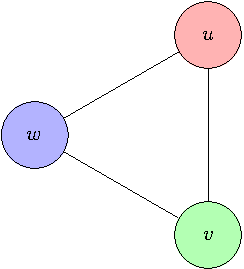
\includegraphics[height=29mm]{Resources/InsertVertexOutside-Example-1.pdf}}
	\quad
	\subfigure[]{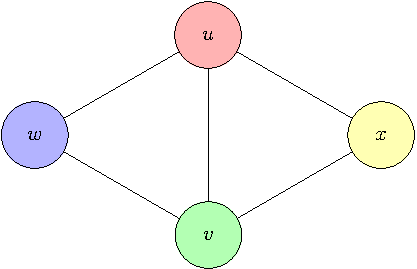
\includegraphics[height=29mm]{Resources/InsertVertexOutside-Example-2.pdf}}
	\qquad
	\subfigure[]{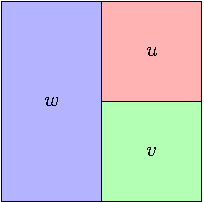
\includegraphics[height=29mm]{Resources/InsertVertexOutside-Example-3.pdf}}
	\quad
	\subfigure[]{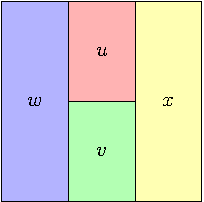
\includegraphics[height=29mm]{Resources/InsertVertexOutside-Example-4.pdf}}
	\caption{A cluster graph and a polygonal dual thereof, before (a, c) and after (b, d) inserting the vertex $x$ on the outer face and connecting it to $u$ and $v$.}
	\label{fig:insert-vertex-outside-example}
\end{figure}

Let $u$ and $v$ be the adjacent vertices on the outer face of the cluster graph and $x$ the new vertex we want to add in the outer face.
Let $p_{uv}$ denote the vertex where the faces $u$ and $v$ meet the outer face of the polygonal dual.
We define $p_u$ and $p_v$ as the first subdivision vertex we encounter when starting at $p_{uv}$ and following the boundary of $u$ and $v$ with the outer face, respectively.
If one of the boundaries consist of only one edge, we place a subdivision vertex at its midpoint and use that vertex as $p_u$/$p_v$.
\Cref{subfig:insert-vertex-outside-illustration-1} shows how these vertices might look for the example from above.
%

\begin{figure}[H]
	\centering
	\subfigure[]{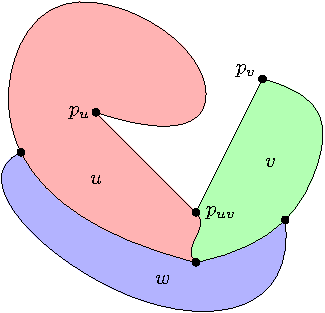
\includegraphics[width=45mm]{Resources/InsertVertexOutside-Illustration-1.pdf}\label{subfig:insert-vertex-outside-illustration-1}}
	\quad
	\subfigure[]{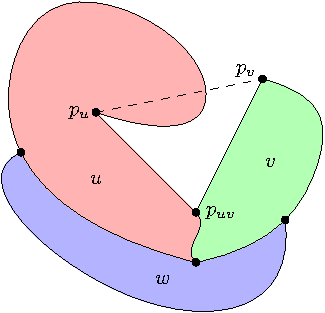
\includegraphics[width=45mm]{Resources/InsertVertexOutside-Illustration-2.pdf}\label{subfig:insert-vertex-outside-illustration-2}}
	\quad
	\subfigure[]{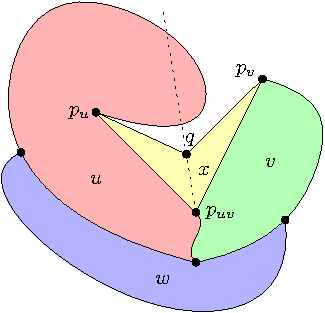
\includegraphics[width=45mm]{Resources/InsertVertexOutside-Illustration-3.pdf}\label{subfig:insert-vertex-outside-illustration-3}}
	\caption{Inserting a face $x$ at the point where the faces $u$ and $v$ meet the outer face.}
	\label{fig:insert-vertex-outside-illustration}
\end{figure}

With $p_u$ and $p_v$ determined, we can create the face $x$ by inserting a path to connect $p_u$ and $p_v$ without introducing edge crossings. Simply inserting an edge between $p_u$ and $p_v$ generally isn't enough, as illustrated in \cref{subfig:insert-vertex-outside-illustration-2}. However, with a single bend in the form of a subdivision vertex $q$, we can guarantee that no edge crossings are being created.

We search for a bend location on the outward-pointing bisector of the angle $\measuredangle_{p_up_{uv}p_v}$, starting at some fixed distance $\epsilon > 0$ and halving the distance until we find a valid location. As the possible bend location moves infinitesimally close to $p_{uv}$, we are guaranteed to find one that doesn't introduce edge crossings. By inserting a vertex at $q$ along with edges $\{q,p_u\}$ and $\{q,p_v\}$, we create an internal face for $x$, as illustrated in \cref{subfig:insert-vertex-outside-illustration-3}.
